\documentclass[amsmath,amssymb,notitlepage,12pt]{revtex4-1}
%\documentclass[12pt]{article}
\usepackage{graphicx}
\usepackage{bm}% bold math
\usepackage{multirow}
\usepackage{booktabs}
\usepackage{verbatim}
\usepackage{hyperref}
\hypersetup{pdftex,colorlinks=true,allcolors=blue}
\usepackage{hypcap}
\usepackage[small,compact]{titlesec}
\begin{document}
\title{HPS Chicane Operations Manual v1.2}
\author{N. Baltzell}
\affiliation{Jefferson Lab}
\date{\today}
\begin{abstract}
    Controls of the HPS chicane are updated for 2016 to simplify operations during shift.  This includes a simplified user interface, automatic retrieval of beam energy, automatic calculations of magnet current setpoints based on~\cite{chicaneSettings}, and EPICS sequencers to energize and disable all HPS chicane magnets with minimal user interaction.  This manual explains the operations of the new interface. 
\end{abstract}
%\hspace*{11.5cm}\texttt{HPS-NOTE 2015-XXX}

%\affiliation{Jefferson Lab}
\maketitle
\tableofcontents
\newpage

\section{Overview}
The new chicane screen is accessiable from the main HPS-EPICS screen, under {\em Magnets}$ \to$ {\em Chicane}, and shown in Figure~\ref{fig:guiChicaneOff}.  It contains a few buttons and many readbacks describe in the following subsections.  Displayed numbers are in units Amps, Gauss, or MeV. 
\begin{figure}[htbp]
    \centering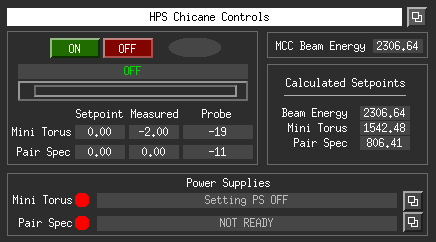
\includegraphics[width=12cm]{pics/guiOFF}
    
    \centering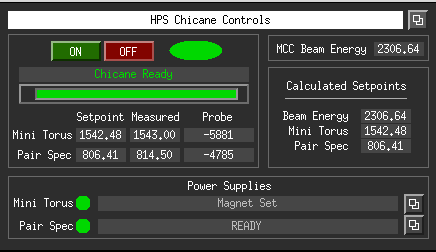
\includegraphics[width=12cm]{pics/guiON}
    \caption{The new chicane screen with both magnets' power supplies off (top), and with chicane energized and ready for 2.306 GeV beam (bottom).\label{fig:guiChicaneOff}}
\end{figure}
\subsection{Buttons}
This GUI contains five buttons:
\begin{enumerate}
    \item The basic {\em ON} and {\em OFF} buttons, which is all the general shift worker should need for controls.
    \item One expert button in the top right corner for customization of chicane setpoints.
    \item Two expert buttons in the bottom right corner that are just links to the magnets' power supplies' old expert screens.
\end{enumerate}
\subsection{Readbacks}
This GUI also contains various readback values:
\begin{enumerate}
    \item In the top left is a global status message and a corresponding progress bar.
    \item Below that are setpoints and measured currents from the magnets' power supplies, and our Hall probes' readback values.
    \item In the top right is the beam energy currently being reported from MCC, and the beam energy and magnet current calculations currently being used by this software to set HPS's magnets.
    \item The bottom portion of the screen is status readbacks from the power supplies.  These are a summary from the magnets' two expert screens.
\end{enumerate}

\section{Shifters Operations}
This is all that shift workers need to operate the chicane:  ``On'' and ``Off''.
\subsection{On}
To turn the chicane on, press the green {\em ON} button.  That will begin a sequence to energize the magnets and eventually bring them to the desired ``calculated'' setpoints shown in the top right of the GUI.  After that is accomplished the main message bar will display ``Chicane Ready'' and you are then ready for beam.  This will take a total of about 40 minutes between the time {\em ON} is pressed and ``Chicane Ready'' is achieved.  The details of the {\em ON} sequence are described in the next section.
\subsection{Off}
To turn the chicane off, press the red {\em OFF} button.  That will begin a sequence to ramp the magents down to zero current and then switch the power supplies off.  Then the main message box should dislay ``OFF''.  This will take a total of about 10 minutes.  The details of the ``OFF'' sequence are described in the next section.

\section{Sequence Details}
\subsection{On}
The ``On'' button will intiate the procedure to go from chicane off to beam ready.  This would normally be done during operations when preparing for first beam after an extended down time or any time the chicane was turned off.
\begin{enumerate}
    \item turn both power supplies on
    \subitem the main message box will display which supply it is turning on
    \item ramp both power supplies up to their max current
    \subitem the progress meter will display progress towards max current
    \item saturate at max current for N minutes
    \subitem the main message box will display the expected remaining time
    \item ramp both power supplies down to their calculated setpoints
    \subitem the progress meter will display the progress towards zero
    \item display ``Ready'' in the main message box
\end{enumerate}
{\em Currently the countdown for saturation time begins when the PairSpec magnet reaches max current.  This was done to conserve time, because Frascati magnets ramp more slowly than the PairSpec but require much less soak time (7 minutes) compared to the PairSpec (30 minutes).}
\subsection{Off}
The ``Off'' button will initiate the procedure to turn the chicane off.  This would normally be done any time the magnets need to be set to zero.
\begin{enumerate}
    \item ramp both power supplies down to zero current
    \subitem the progress meter will display progress towards zero current
    \item turn both power supplies off
    \subitem the main message box will display which supply it is turning off
    \item display ``OFF'' in the main message box
\end{enumerate}

\newpage
\section{Expert Operations}
The expert gui is a work in progress, written mostly in anticipation of what may be needed in the future. 
\begin{enumerate}
\item The topmost section is of most importance, calculating the magnet currents from the MCC beam energy.  This uses the relationship between beam energy and magnet currents given in~\cite{chicaneSettings}.
\item
    The second section allows to choose your own beam energy, and then calculate the magnet currents based on beam energy given in~\cite{chicaneSettings}.
\item
The third sections allows to manually scan the magnet currents by adjusting only the beam energy, in accordance with the equations given in~\cite{chicaneSettings}.  This could be useful for a manual scan of chicane settings.
\item
The fourth section just allows to manually input setopints to the power supplies.  This is identical to manually inputting the currents in the expert screens for the individual power supplies.
\item
The last section is some parameters on the sequencer: time to hold for saturation and tolerance to for the sequencer to think measured currents are acceptable.
\end{enumerate}
\begin{figure}[htbp]\centering
    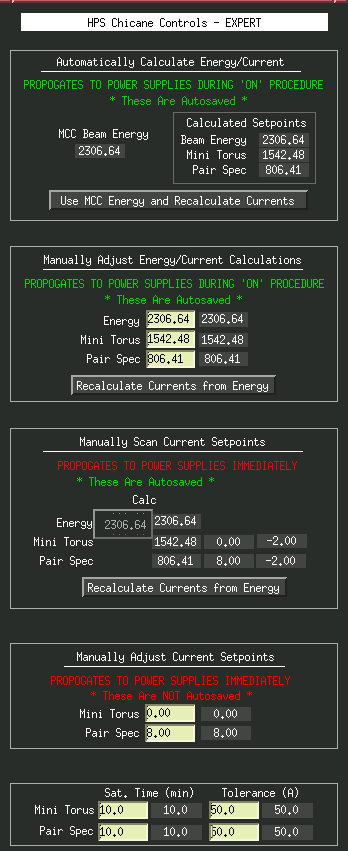
\includegraphics[height=18cm]{pics/expert}
    \caption{\label{}}
\end{figure}


\bibliography{ChicaneManual}
\end{document}

